\section{Resources}
\label{sec:api_resources}

Before introducing networks, we first need to introduce Brel's approach to resources.
Resources are XBRL's way of representing metadata, 
which links to other elements of the an XBRL report using networks.

Like report elements and characteristics before them, resources share a common interface.
There are three types of resources in XBRL - label, reference and definition.
Each of these types of resources is represented by a different class in Brel.
The class diagram in figure \ref{fig:brel_resource_classes} illustrates the relationship between the different resource classes.

\begin{figure}[H]
    \centering
    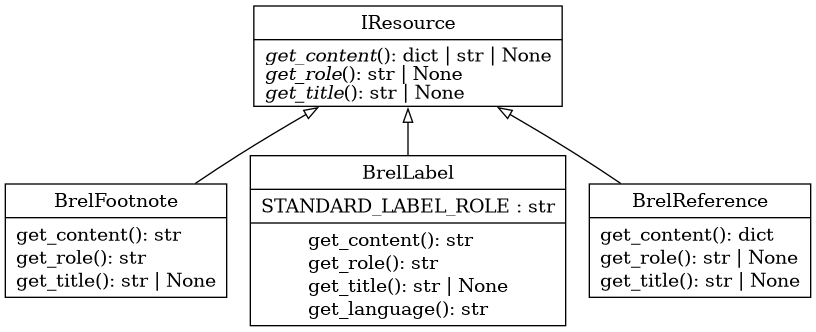
\includegraphics[width=\textwidth]{images/brel_resource_classes.png}
    \caption{UML diagram of the resource classes in Brel}
    \label{fig:brel_resource_classes}
\end{figure}

\subsection{IResource}

Resources consist of three parts - a role, a title and content.

The role acts as a type identifier for the resource.
For example, even though each XBRL label is represented using a \texttt{BrelLabel} object, 
there are different types of labels.
Different types of labels are distinguished using their role.
As the name suggests, the \texttt{get\_role} method returns the role of the resource. 

Next up is the content of the resource, which is accessed using the \texttt{get\_content} method.
Usually, the content is a string.
For references however, the content is embedded XML.
Since Brel intends to remove any XML dependencies, it returns the embedded XML as a dictionary instead. 

% The title is a human-readable description of the resource.
The title, accessed using the \texttt{get\_title} method, is a human-readable description of the resource.
For labels, the title is often omitted, since the label itself is already short and descriptive.
However, the content of a resource can be arbitrarily long, which is why XBRL supports titles.

\section{Labels and Footnote}

Footnotes and labels are two types of resources that are used to link to other elements of an XBRL report.
Even though they have their own classes, they are very similar from an API perspective.

Both of them implement the \texttt{IResource} interface.
The methods \texttt{get\_role}, \texttt{get\_title} and \texttt{get\_content} function virtually the same.
Unlike their common interface, labels and footnotes have an additional method called \texttt{get\_language}.
The \texttt{get\_language} method returns the language of the resource.

\subsubsection{References}

References are the third type of resource in XBRL.
They are used to link XBRL reports to external resources.
References are represented by the \texttt{Reference} class in Brel and implement the \texttt{IResource} interface.
They do not have a \texttt{get\_language} method like labels and footnotes do.
Another difference is that the content of a reference is a dictionary instead of a string.

Now that we have covered resources, we can finally introduce networks.
